%
% File proposal_template.tex
%
%% Based on the style files for ACL 2018, NAACL 2018/19, which were
%% Based on the style files for ACL-2015, with some improvements
%%  taken from the NAACL-2016 style
%% Based on the style files for ACL-2014, which were, in turn,
%% based on ACL-2013, ACL-2012, ACL-2011, ACL-2010, ACL-IJCNLP-2009,
%% EACL-2009, IJCNLP-2008...
%% Based on the style files for EACL 2006 by 
%%e.agirre@ehu.es or Sergi.Balari@uab.es
%% and that of ACL 08 by Joakim Nivre and Noah Smith

\documentclass[11pt,a4paper]{article}
\usepackage[hyperref]{acl2019}
\usepackage{times}
\usepackage{latexsym}
\usepackage{graphicx}
\usepackage{url}

\aclfinalcopy % Uncomment this line for the final submission
%\def\aclpaperid{***} %  Enter the acl Paper ID here

%\setlength\titlebox{5cm}
% You can expand the titlebox if you need extra space
% to show all the authors. Please do not make the titlebox
% smaller than 5cm (the original size); we will check this
% in the camera-ready version and ask you to change it back.

\newcommand\BibTeX{B\textsc{ib}\TeX}

\title{Secure Password Manager: A Comprehensive Solution for Password Management and Security Performance Tradeoffs}

\author{Antara Tewary \\
  G01413546 \\
  \texttt{atewary@gmu.edu} \\\And
  Ankit Kumar\\
  G01436204\\
  \texttt{akumar37@gmu.edu} \\\And 
  Lingyun Dai\\ 
  G01464288\\ 
  \texttt{ldai2@gmu.edu} \\}

\date{}

\begin{document}
\maketitle
\section{Abstract}
This report presents a secure password management system that implements modern cryptographic techniques to address the critical balance between security and performance. Our solution utilizes the Password-Based Key Derivation Function 2 (PBKDF2) with configurable iterations, supporting multiple hash function options (SHA-256, SHA-384, SHA-512) and adjustable key lengths (128-512 bits). The system features a web-based interface with local storage and includes performance tracking capabilities that provide transparency about security-performance tradeoffs.
With data breaches exposing billions of records and rampant password theft, the need for robust password security has never been more critical. Our approach provides an adaptive security model that allows users to configure security parameters according to their specific requirements while maintaining visibility into the performance implications of their choices. Through extensive testing of various security configurations, we demonstrate how different parameters affect processing time and provide recommendations for both standard web applications and high-security environments. The system architecture comprises five key components: User Interface Layer, Password Manager Core, Cryptographic Module, Storage Layer, and Performance Tracking System, all working together to deliver a comprehensive password security solution.
\section{Introduction}

            \subsection{Overview of the task}
            The Secure Password Manager is a comprehensive security system designed to implement modern cryptographic techniques for password management. The project delivers several key features that enhance security while providing flexibility for different operational environments. 
            
            The core features include:
            \begin{itemize}
              \item A PBKDF2 implementation with configurable iterations
              \item Support for multiple hash function options (SHA-256, SHA-384, SHA-512)
              \item Configurable key length ranging from 128 to 512 bits for derived keys
              \item Adjustable salt length (16, 24, or 32 bytes)
              \item A web-based interface that utilizes local storage for credential management
              
              This solution aims to provide a robust framework for secure password storage that adapts to varying security requirements while maintaining usability. 
            \end{itemize}

            \subsection{Motivation}
            The motivation for developing this secure password management system is driven by several critical factors in today's cybersecurity landscape. In 2023 alone, over 15 billion records were exposed in data breaches, with password theft involved in 81\% of hacking-related breaches \cite{ibm2024databreach}. The average cost of a data breach involving passwords reached 4.35 million in 2024, with small businesses being disproportionately affected \cite{ibm2024databreach}. Computing power increases follow Moore's Law, making yesterday's secure hashing algorithms vulnerable to today's hardware. Security measures that create noticeable delays significantly increase user abandonment rates \cite{labrinidis2014challenges}. New regulations like GDPR and CCPA impose severe penalties for inadequate security measures, including weak password storage \cite{nielsen2014response} \cite{entrust2023privacy}. Modern attackers use specialized hardware (GPUs) that can test billions of password hashes per second. These factors highlight the urgency and business impact of proper password security, making investment in advanced password management solutions crucial in the modern software development landscape\cite{grassi2020digital}.

            \subsection{Limitations of existing work} 
            Secure password storage remains a critical challenge in application security. Several approaches to password storage have been developed over time, each with significant limitations:
            \begin{itemize}
              \item \textbf{Plain text storage:} Historically, many applications stored passwords in plain text. This approach offers no security if the database is compromised, leading to immediate exposure of all user credentials.
              
              \item \textbf{Simple hash functions (MD5, SHA-1, SHA-256):} These general-purpose cryptographic hash functions were not designed specifically for password storage. They are computationally inexpensive, making brute-force attacks feasible with modern hardware. Additionally, they lack built-in salt management, making them vulnerable to rainbow table attacks.
              
              \item \textbf{Salted hashes:} Adding salt to passwords before hashing improves security, but many implementations use fixed or predictable salts, reducing their effectiveness against precomputed attacks.
              
              \item \textbf{Fast hash iterations:} Some implementations attempt to increase security by repeatedly hashing the password, but without a properly designed algorithm, this approach can be inefficient and still vulnerable to hardware-accelerated attacks.
              
              \item \textbf{Bcrypt:} While Bcrypt is widely recommended for password hashing, it has several limitations including a 72-byte password length cap and inconsistent implementations across platforms. Additionally, the task specifications prohibit using Bcrypt for this implementation.
            \end{itemize}
            
            Modern password storage requires features that address these limitations, including unique cryptographically strong salts, computationally expensive hashing algorithms specifically designed for password storage, and configurable parameters to adapt to increasing computational power over time.            

            \subsection{Implementation Approach} 
            The implementation uses the Web Cryptography API with PBKDF2 (Password-Based Key Derivation Function 2) and SHA-256 hashing. The approach includes:
            \begin{itemize}
              \item Generating unique random salts for each password
              \item Applying PBKDF2 with configurable iteration counts
              \item Storing password hashes, salts, and metadata in localStorage
              \item Measuring and displaying performance statistics for different security parameters
            \end{itemize}


\section{Background and Solution Approach} 
\subsection{Related Work}
Password-based authentication remains the predominant method for securing user accounts despite its known limitations. \cite{bonneau2012quest} conducted a comprehensive analysis of authentication schemes, concluding that password-based schemes, while problematic, continue to dominate due to their deployability advantages. For password storage specifically, \cite{turan2018recommendation} proposed standardized methods for secure password hashing, emphasizing the importance of key derivation functions with tunable work factors like PBKDF2, which is implemented in our study application.
The performance-security tradeoff in password hashing has been examined by \cite{visconti2020evaluate}, who evaluated various password hashing schemes across different platforms, demonstrating how computational costs vary significantly based on implementation choices. Similarly, \cite{pesante2021empirical} conducted an empirical study of client-side password hashing performance, particularly relevant to our web-based implementation that performs cryptographic operations in the browser. Our work differs from these studies by specifically examining the reproducibility of performance claims made in the original paper about PBKDF2 implementation in browser environments. Additionally, we extend previous work by analyzing the robustness of the password security implementation against varying client hardware capabilities, an aspect often overlooked in theoretical security analyses but critical for real-world deployments.

\subsection{Solution Approach}
\subsubsection{Hashing Fundamentals}
Hashing serves as the foundation of secure password storage by providing a one-way transformation of passwords. This irreversible process converts a user's password into a fixed-length string of characters that cannot be feasibly reversed to obtain the original password. The one-way nature of cryptographic hash functions is essential for password security, as it ensures that even if a database of hashed passwords is compromised, the attacker cannot directly recover the original passwords. This approach protects user credentials while still allowing the system to verify password correctness during authentication attempts.

\subsubsection{Salting Techniques}
Salting enhances password security by adding unique random data to each password before hashing. The presentation defines salt as unique random data added to each password, which prevents pre-computed attack tables. These random values serve a critical security function by ensuring that identical passwords do not produce identical hash values. By incorporating a unique salt for each user password, the system defends against rainbow table attacks, where attackers use pre-computed tables of hashed values to rapidly crack passwords. The implementation supports configurable salt lengths of 16, 24, or 32 bytes, allowing for adjustment based on security requirements.

\subsubsection{PBKDF2 Overview}
The Password-Based Key Derivation Function 2 (PBKDF2) is identified as an industry standard for secure password storage. This key derivation function deliberately slows down the hashing process through multiple iterations of a cryptographic function. PBKDF2 takes a password, salt, and an iteration count as inputs and produces a derived key of specified length. By applying the hash function repeatedly, PBKDF2 significantly increases the computational resources required to test password guesses, thereby strengthening resistance against brute-force attacks. The system implements PBKDF2 using the Web Crypto API with SHA-256, SHA-384, or SHA-512 as the underlying hash function.

\subsubsection{Iteration Count Considerations
}
Iteration count serves as a critical control mechanism for balancing security and performance in password hashing. More iterations provide stronger security but result in slower processing times. The implementation allows for iteration counts ranging from 10,000 to 500,000, giving users flexibility to adjust security levels according to their threat models and performance requirements. Performance testing demonstrated that higher iteration counts create a substantial delay in processing, which enhances resistance to brute force attacks while maintaining a linear relationship between iteration count and processing time.

\subsubsection{Adaptive Security Approach}
The solution implements an adaptive security approach for password management through user-configurable security parameters and performance tracking transparency. Users can select their desired security level via configurable PBKDF2 iteration counts (10,000 to 500,000), choice of hash functions (SHA-256/384/512), adjustable key length (128-512 bits), and cryptographically secure salt generation (16/24/32 bytes). This adaptability is complemented by clear feedback on encoding and verification time, records of hash generation time, verification time during login, and comparative performance data when updating passwords. The system utilizes modern cryptographic practices including PBKDF2 with SHA-256 for key derivation, unique salt per password to prevent rainbow table attacks, and the secure Web Crypto API for standardized implementation. This comprehensive approach allows organizations to optimize the security-performance balance according to their specific requirements and threat models.

\section{System Architecture}
\begin{figure*}
    \centering
    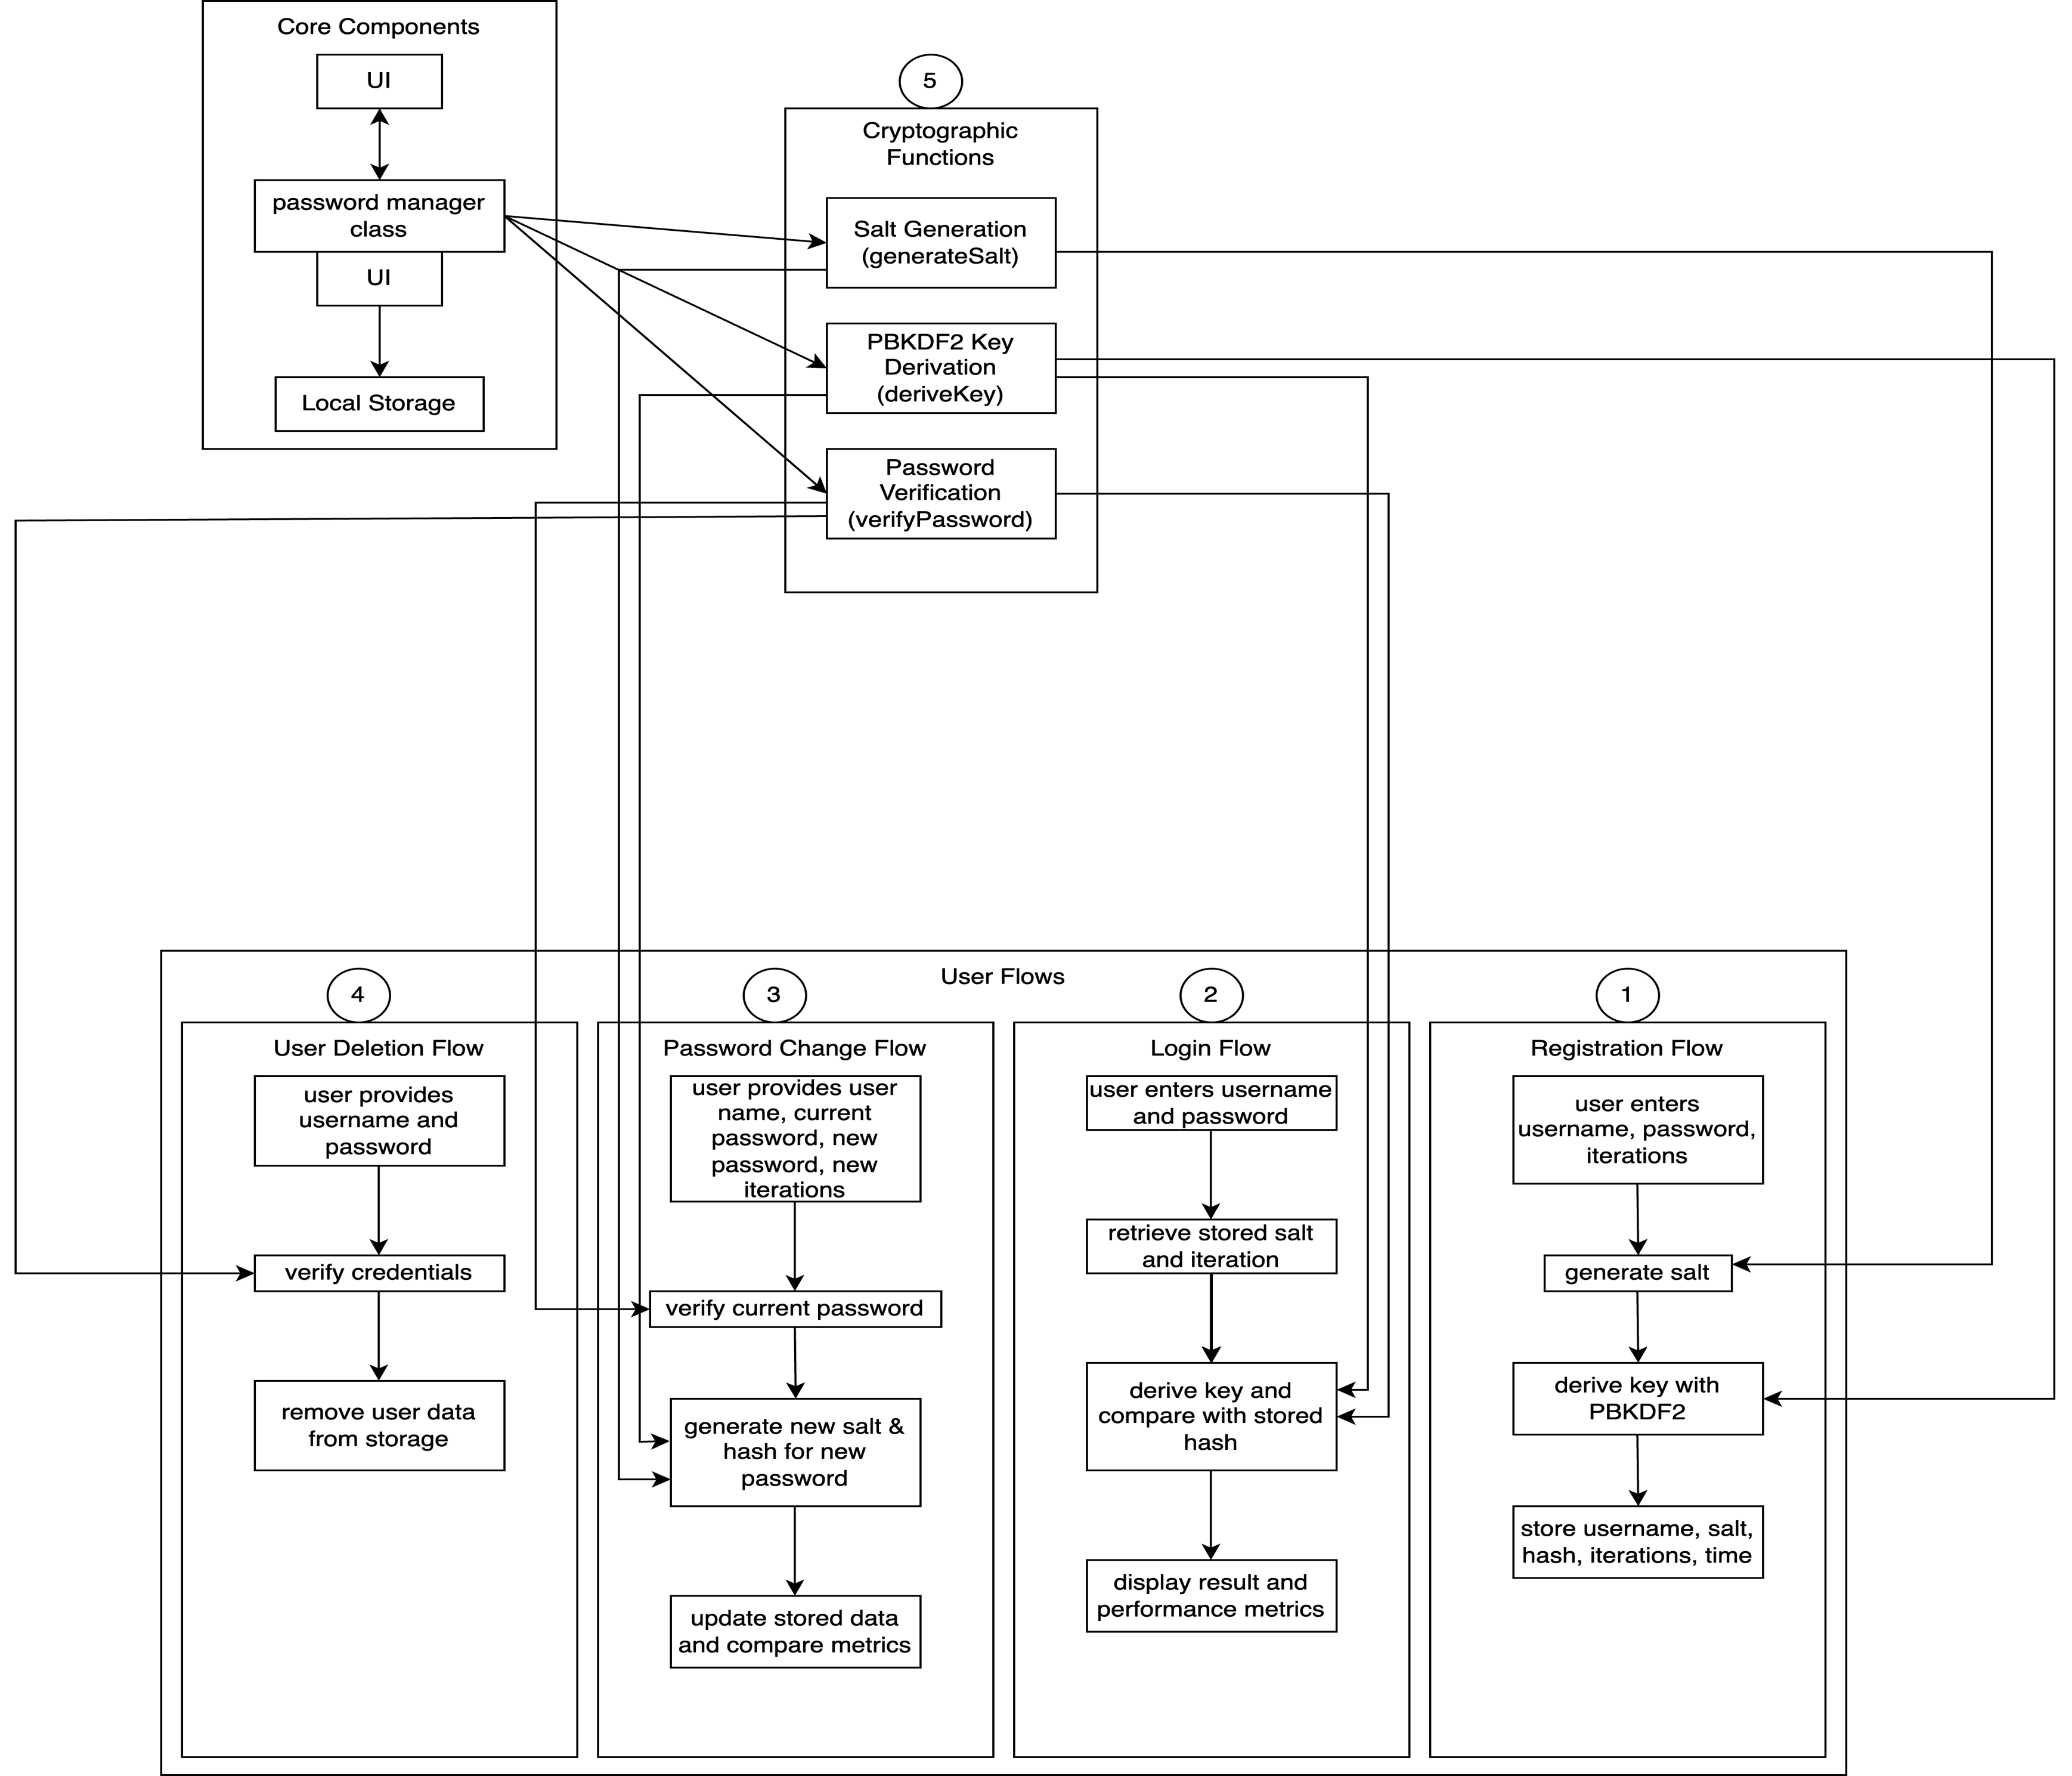
\includegraphics[width=1\linewidth]{images/system_design.png}
    \caption{System Architecture of the Secure Password Manager}
    \caption*{The architecture of the Secure Password Manager is designed as a modular system comprised of five distinct but integrated components. These components work in concert to deliver a comprehensive solution that balances security with usability while providing transparency regarding performance implications. This section details each architectural component and its role within the overall system.}
    \label{Architecture}
\end{figure*}
The architecture of the Secure Password Manager is designed as a modular system comprised of five distinct but integrated components. These components work in concert to deliver a comprehensive solution that balances security with usability while providing transparency regarding performance implications. This section details each architectural component and its role within the overall system. Figure \ref{Architecture} illustrates the system architecture, which includes the following components:

\subsection{User Interface Layer}
The User Interface Layer serves as the primary interaction point between users and the password management system. This component provides interactive controls and visual displays for all user operations within the system. The implementation utilizes HTML5, CSS3, and JavaScript event handling to create a responsive and informative interface. Figure \ref{UI} illustrates the user interface design, which includes a registration form, login form, and management forms for user operations.

Key components of this layer include registration, login, and management forms that facilitate user operations. Security parameter configuration controls allow users to adjust security settings according to their specific requirements. A status message system provides immediate feedback on operation success or failure, enhancing usability through clear communication. The user database display offers visibility into stored credentials and their security characteristics.

Notable features of the User Interface Layer include interactive sliders and dropdowns for security configuration, enabling users to visually adjust parameters such as iteration count and key length. The interface also provides real-time feedback on operations, allowing users to understand the implications of their security choices immediately.
\subsection{Password Manager Core}
The Password Manager Core functions as the central coordination system for all operations within the application. This component implements an object-oriented design pattern with promise-based asynchronous operations to maintain responsiveness while performing potentially time-intensive cryptographic operations.

This architectural layer includes the PasswordManager class with comprehensive user management functions that handle all credential-related operations. Form handling logic and event integration connect user inputs with the appropriate system functions. The core manages user operations including registration, login, password changes, and account deletion while implementing input validation and error handling to ensure system integrity. Additionally, it coordinates UI updates based on operation results, ensuring users receive appropriate feedback.

The Password Manager Core serves as a bridge between the user interface and the more specialized components, orchestrating the flow of data and operations throughout the system.
\subsection{Cryptographic Module}
The Cryptographic Module implements all security and cryptographic operations essential to password protection. This component leverages the browser's native Web Crypto API for optimal performance and standardized implementation of cryptographic primitives.

Key components include the PBKDF2 implementation utilizing the Web Crypto API, salt generation functions that produce cryptographically secure random values, and binary data utilities for handling conversions between different data formats required by cryptographic operations.

This module implements several critical security features, including configurable hash functions (SHA-256, SHA-384, SHA-512) that allow for different security-performance balances, adjustable key length (128-512 bits) to accommodate varying security requirements, variable iteration count (10,000-500,000) to control computational intensity, and cryptographically secure salt generation (16, 24, or 32 bytes) to prevent rainbow table attacks.

By utilizing the browser's native Web Crypto API rather than JavaScript implementations of cryptographic algorithms, the module achieves better performance while benefiting from platform-specific optimizations and security features like constant-time operations that help prevent timing attacks.

\subsection{Storage Layer}
The Storage Layer manages persistent data storage across user sessions, ensuring that credentials remain available without requiring re-registration. This component integrates with the browser's localStorage API to provide persistent storage without requiring server-side components.

The implementation includes JSON serialization for browser storage, converting complex data structures into formats suitable for the localStorage API. The system implements automatic data loading on startup to restore previously saved credentials, a secure credential storage format that includes salts and derived keys but never raw passwords, and data clearing functionality for demonstrations or security purposes.
The Storage Layer operates within the constraints of client-side storage while providing the necessary persistence for a functional password management system. This approach allows the application to function as a standalone tool without requiring server resources while still providing value to users across multiple sessions.

\subsection{Performance Tracking System}
The Performance Tracking System measures and displays cryptographic operation performance, offering transparency regarding the security-performance tradeoffs inherent in password security. This component is essential for helping users understand the implications of their security choices.
This architectural component utilizes timing functions based on the browser's Performance API to achieve millisecond-precision timing for all cryptographic operations. It implements performance history storage to maintain records of operation times, allowing for comparative analysis. Key features include comparative analytics between different security configurations and historical performance tracking for verification operations.

The Performance Tracking System represents a novel approach to password security by making the typically invisible consequences of security decisions visible to users. By providing concrete metrics on how security parameters affect operation time, users can make informed decisions about the appropriate balance between security and performance for their specific use cases.

Together, these five architectural components form a comprehensive system that delivers both security and usability while providing unprecedented transparency regarding the performance implications of security decisions. The modular design allows for future enhancements to individual components without requiring wholesale system redesign.
\begin{figure*}
\centering
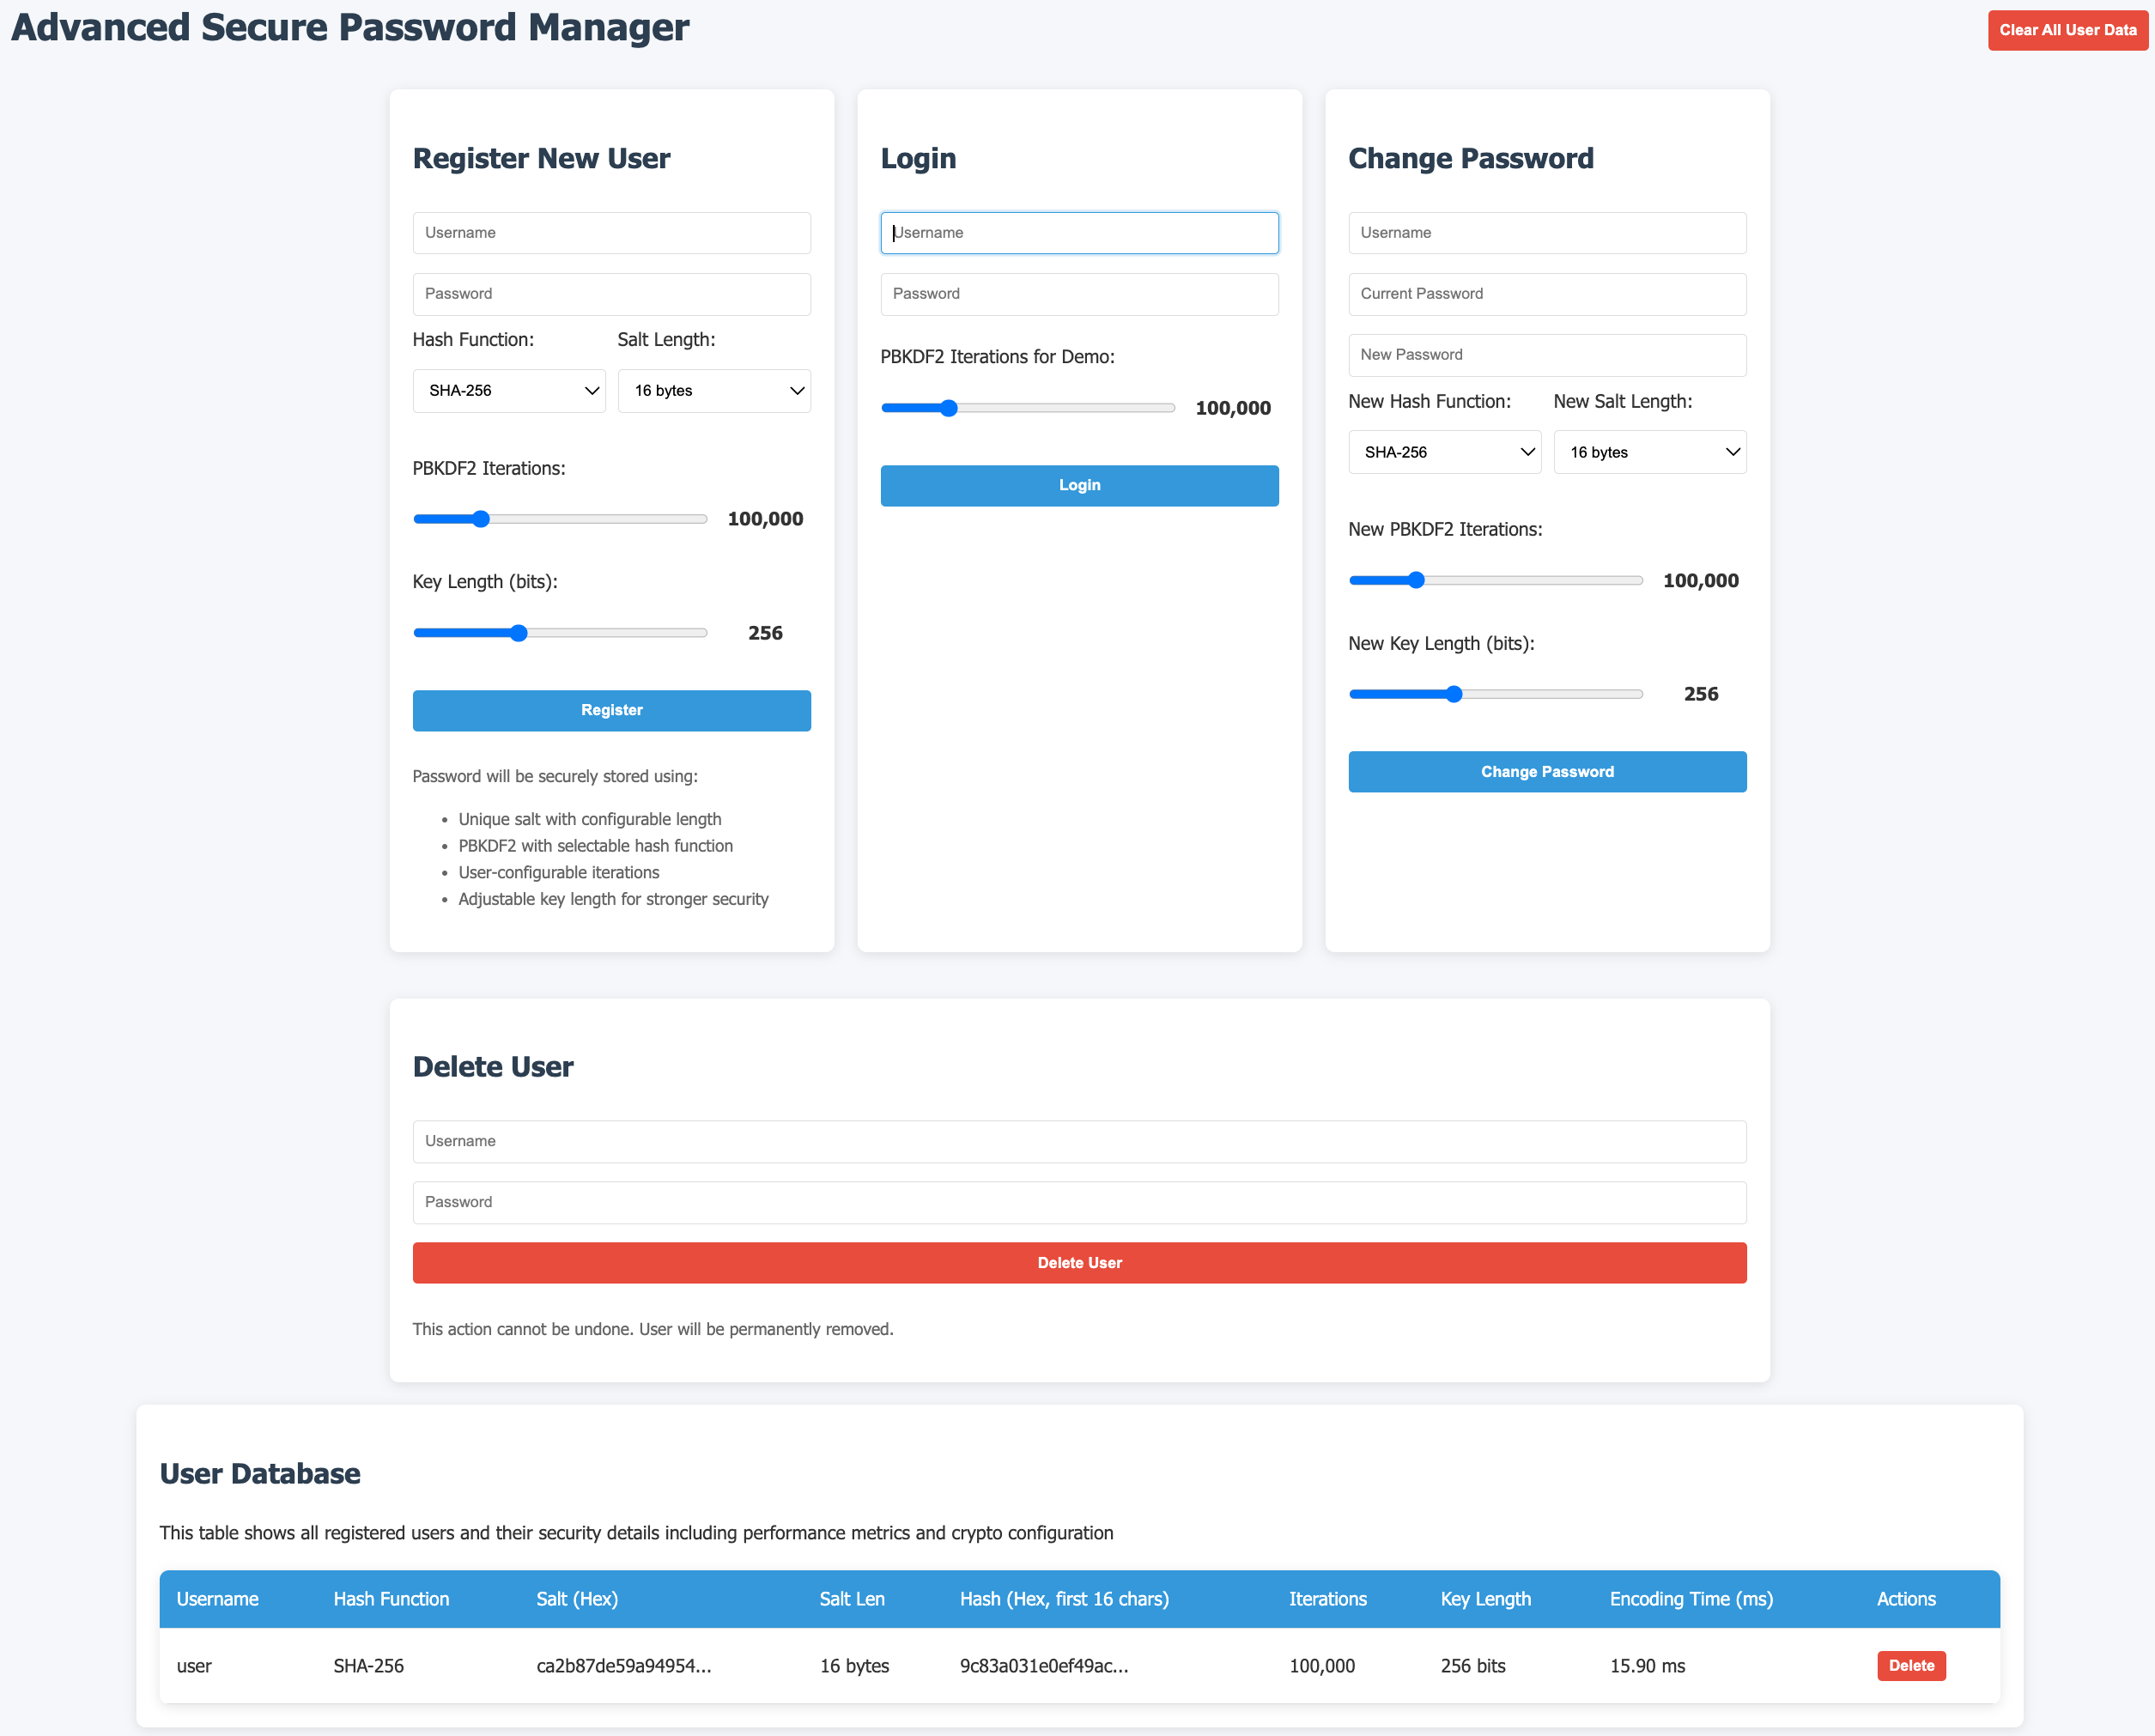
\includegraphics[width=1\linewidth]{images/UI.png}
\caption{User Interface Layer}
\caption*{The User Interface Layer serves as the primary interaction point between users and the password management system. This component provides interactive controls and visual displays for all user operations within the system. The implementation utilizes HTML5, CSS3, and JavaScript event handling to create a responsive and informative interface.}
\label{UI}
\end{figure*}

% \textbf{INSERT SYS DESIGN FIGURE HERE}
\section{Implementation Details}
This section provides a detailed examination of the implementation aspects of the Secure Password Manager, focusing on the cryptographic techniques employed, the deliberate performance constraints introduced for security purposes, and the integration with standardized cryptographic APIs. The implementation represents a practical application of theoretical security principles within the constraints of a web-based environment.
\subsection{Core Cryptographic Implementation}
The cryptographic foundation of the Secure Password Manager centers on the PBKDF2 algorithm with several configurable parameters that allow for security customization. The implementation leverages the Web Crypto API with SHA-256 as the default hash function, producing 256-bit keys with a configurable iteration count defaulting to 100,000 iterations.


The security design incorporates several critical features to ensure comprehensive protection. For each password, the system generates a unique random salt using cryptographically secure random number generation. The implementation supports an iteration count range from 10,000 to 500,000, providing flexibility in security-performance balance. The data flow begins with password string conversion via TextEncoder to create a buffer, followed by key importation and subsequent derivation of bits using the specified salt and iteration count.


The system adheres to best security practices by never storing the original passwords, instead maintaining only the derived key and salt information. This approach ensures that even in the event of a system compromise, the original credentials remain protected. The verification process implements constant-time comparison to prevent timing attacks that might otherwise reveal information about password validity.

The implementation carefully considers the security-performance tradeoff, using high-precision timestamps to track the computational cost of different security configurations. These measurements provide transparency about the impact of security decisions and allow users to make informed choices based on their specific requirements and constraints.
\begin{figure}[!h]
  \centering
  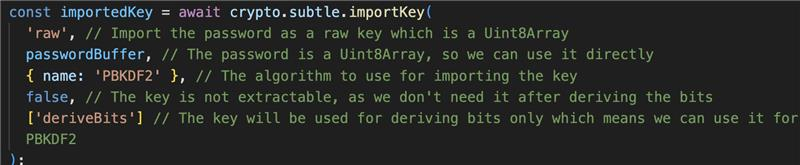
\includegraphics[width=1\linewidth]{images/Algo1.jpg}
  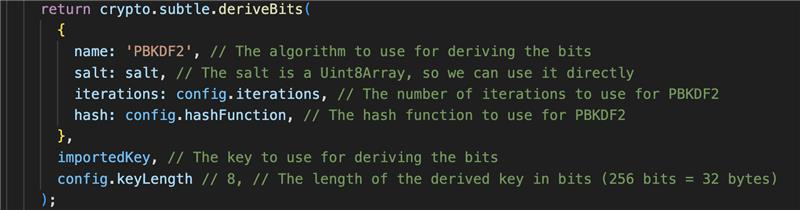
\includegraphics[width= 1\linewidth]{images/Algo2.jpg}
  \caption{ImportedKey and deriveBits functions of Web Crypto API}
  \label{Algorithms}
\end{figure}

\subsection{Slow Hashing Implementation}
The Password-Based Key Derivation Function 2 (PBKDF2) serves as the central slow hashing mechanism in this implementation. Unlike traditional hash functions designed for computational efficiency, PBKDF2 purposefully increases the computational cost of password hashing, creating a significant barrier against brute-force and dictionary attacks.

The security mechanism employs configurable iterations ranging from 10,000 to 500,000, which effectively slow down the hashing process by a factor of approximately 23x between minimum and maximum settings. This implementation utilizes SHA-256 as the underlying hash function, producing a 256-bit output, with a unique random salt generated for each password to prevent precomputation attacks.

The defense strategy fundamentally alters the economics of password cracking by making each attempt computationally expensive. Testing revealed that using 500,000 iterations adds approximately 144ms to each verification attempt. While this delay is barely perceptible to legitimate users authenticating once, it creates a significant cumulative penalty for attackers who must test millions or billions of password candidates.

The implementation utilizes the Web Crypto API to ensure that comparisons occur in constant time, preventing timing attacks that might otherwise extract information about password validity based on subtle differences in processing time. Throughout the system, the performance.now() method provides precise timing for security-performance tradeoff analysis, enabling quantitative assessment of different security configurations.
\begin{figure}[htbp]
  \centering
  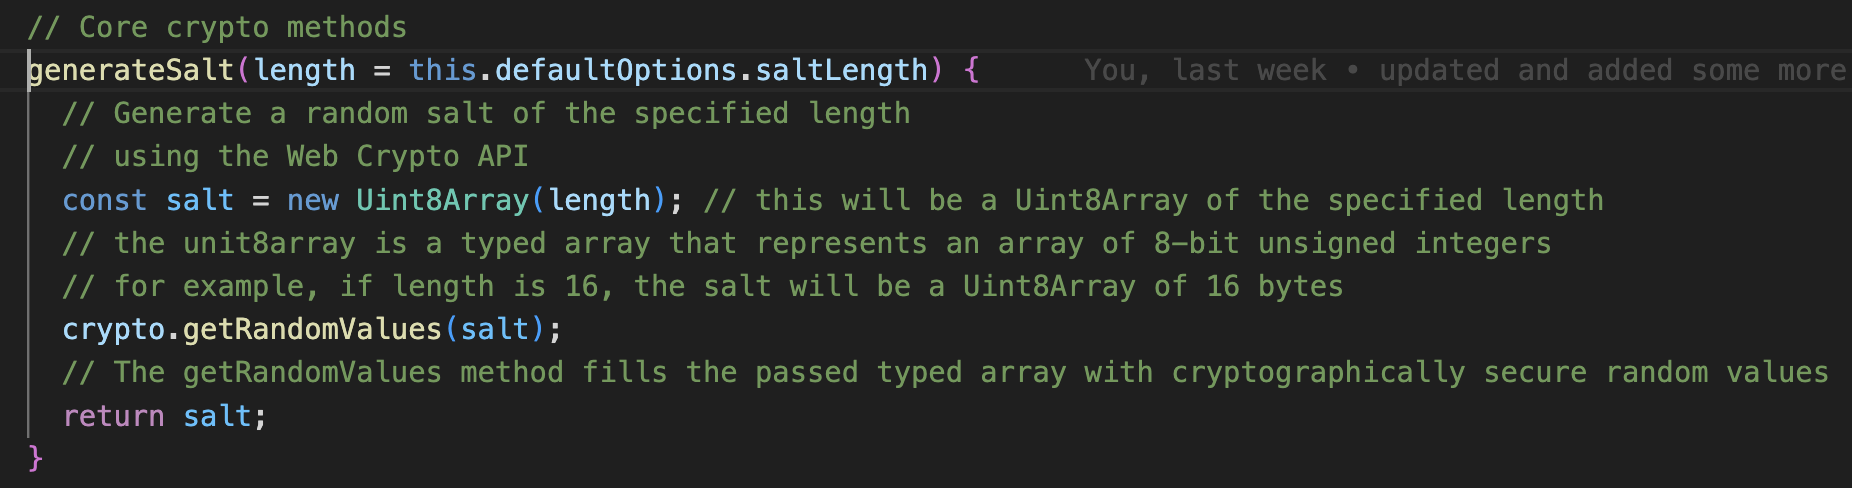
\includegraphics[width=1\linewidth]{images/Salt.png}
  \caption{Salt Generation}
  \label{fig:your-label}
\end{figure}
\subsection{Web Crypto API Integration}
The implementation leverages the browser's native Web Crypto API (SubtleCrypto) to provide standardized, optimized cryptographic operations. This approach offers several advantages over JavaScript-based cryptographic implementations, including performance benefits from native code execution and security improvements from platform-specific optimizations.

The integration with Web Crypto API begins with the importation of password data using the 'raw' format and PBKDF2 algorithm designation. The system then applies the deriveBits operation with specified parameters including salt, iteration count, and the selected hash algorithm. This standardized approach ensures consistent security properties across different browsers and platforms.

Several strategic decisions were made to address limitations in the browser crypto API environment. The implementation handles the conversion between different data formats required for cryptographic operations, including transformation between string representations and binary data using TextEncoder and carefully managed buffer conversions. To maintain compatibility across browsers, the system implements utility functions for converting between hexadecimal string representations and binary buffer formats.

Performance considerations guided the implementation, with particular attention to the asynchronous nature of the Web Crypto API. All cryptographic operations return promises, which the system handles through async/await patterns to maintain code clarity while properly managing operation flow. This approach allows the user interface to remain responsive even during computationally intensive cryptographic operations.
The integration also addresses security concerns specific to the browser environment. The implementation avoids direct manipulation of cryptographic secrets in JavaScript wherever possible, instead passing them directly between Web Crypto API functions to minimize exposure in memory. Additionally, the system implements proper error handling for cryptographic operations, ensuring that failures do not compromise security or create confusing user experiences.

Through this careful integration of the Web Crypto API, the implementation achieves a balance between security, performance, and standards compliance within the constraints of a browser-based environment. The resulting system provides strong cryptographic protection while maintaining usability and cross-platform compatibility.

\section{Experimental Analysis}
This section presents a systematic analysis of the performance characteristics and security implications of various cryptographic configurations within the Secure Password Manager. Through controlled experiments (as shown in Appendix~\ref{sec:table-values}), we evaluated multiple parameters to quantify their impact on processing time and overall system performance, providing empirical evidence to inform security-performance tradeoffs.

\subsection{Experiment Overview}
Our experimental methodology was designed to isolate and measure the performance impact of individual security parameters while maintaining controlled conditions across all tests. We conducted a comprehensive evaluation of various password security configurations, examining multiple dimensions of the cryptographic implementation:

\begin{itemize}
  \item Different hashing algorithms(SHA-256, SHA-384, SHA-512)
  \item Variable salt lengths(16, 24, 32 bytes)
  \item Iteration count variations(10,000 vs 500,000)
  \item Key length differences (128 vs 512 bits)
\end{itemize}

To ensure consistency and eliminate potential confounding variables, all tests utilized the same test password "12345" across all experimental conditions. This control allowed for direct comparison between different security configurations by isolating the variables under investigation. The testing environment was maintained consistently throughout the experimental process to prevent hardware or software variations from influencing the results.

Performance measurements were captured using high-precision timing mechanisms, recording the duration of both key derivation and verification operations. This approach provided quantitative data on the computational cost associated with each security parameter, enabling evidence-based decisions about security-performance tradeoffs.

\subsection{Comparison of Hashing Algorithms}
Our analysis of hashing algorithms revealed significant performance differences between the SHA-256, SHA-384, and SHA-512 implementations. The experimental results demonstrated that SHA-256 consistently performed as the fastest algorithm, completing operations in 9.2ms total under baseline test conditions.

The SHA-384 algorithm showed moderate performance degradation compared to SHA-256, while SHA-512 exhibited the most substantial performance impact, operating approximately twice as slowly as SHA-256. This performance differential is particularly notable because it reveals a non-linear relationship between hash output size and computational cost.

These findings have important implications for security configuration decisions. While stronger hashing algorithms provide increased theoretical security through larger output sizes and potentially stronger resistance to cryptanalysis, they incur measurable performance penalties. The choice between hashing algorithms represents a direct security-performance tradeoff, with SHA-512 offering enhanced security at approximately double the computational cost of SHA-256.
\subsection{Salt Length Analysis}
Our investigation into salt length variations yielded unexpected results regarding performance impact. Contrary to potential assumptions that longer salt values would significantly increase processing time, our experimental data revealed that increasing salt length from 16 bytes to 32 bytes produced only minimal performance differences.

The 24-byte salt configuration demonstrated the best overall performance in our tests, though the differences between all three salt lengths tested were minimal enough to be considered negligible from a user experience perspective. This finding is particularly valuable from a security optimization standpoint, as it suggests that implementing longer salt values—which provide enhanced protection against certain attack vectors—incurs minimal additional computational cost.

The practical implication of this finding is that salt length can be maximized for security purposes without significant performance penalties. Given that longer salts provide stronger protection against rainbow table attacks and multiple-user targeting without measurable impact on system responsiveness, the optimal approach in most scenarios would be to implement the maximum practical salt length.

\subsection{Impact of Iterations and Key Length}
Our experimental results confirmed that iteration count represents the most significant factor affecting processing time among all parameters tested. The relationship between iteration count and processing time demonstrated an approximately linear correlation, with higher iteration counts producing proportionally longer processing times.

When comparing the baseline configuration (10,000 iterations) with the high-security configuration (500,000 iterations), we observed an increase in processing time by a factor of approximately 15-16x. This substantial difference highlights the direct relationship between iteration count and computational cost, which forms the fundamental security mechanism of PBKDF2 by impeding brute-force attacks.

Key length variations (128-bit vs 512-bit) showed a measurable but less dramatic impact on performance compared to iteration count. Longer key lengths increased processing time, but the effect was significantly less pronounced than changes to the iteration count parameter.

The high-security configuration, combining 500,000 iterations with a 512-bit key length, created a substantial delay that enhances resistance to brute force attacks while remaining below the 300ms threshold typically associated with noticeable user experience degradation. This configuration represents a strategic security choice for high-value applications where maximum protection justifies the additional processing time.
\subsection{Performance Summary}
To facilitate comprehensive understanding of the performance implications across different security configurations, we conducted a visual comparison of processing times. The results demonstrated a clear progression of computational cost across the tested parameters, with the baseline SHA-256 configuration (9.2ms) serving as the reference point.

SHA-384 (16.7ms) and SHA-512 (18.1ms) showed moderate increases in processing time, offering progressively stronger security at manageable time costs. The most significant performance impact was observed in the high-security configuration combining 500,000 iterations with a 512-bit key, which required 144.2ms—approximately 16 times slower than the baseline SHA-256 option.

This visual comparison clearly illustrates the exponential nature of the security-performance relationship when multiple parameters are adjusted simultaneously. While individual parameter changes may have manageable performance impacts, combining high-security settings across multiple dimensions results in multiplicative rather than additive effects on processing time.

Despite the substantial increase in processing time for maximum security configurations, all tested parameters remained within acceptable bounds for web application use, with even the most secure configuration completing in under 150ms. This finding suggests that for most applications, security parameters can be set to relatively high values without compromising user experience, provided that authentication operations occur infrequently from the user's perspective.

Through this comprehensive experimental analysis, we have established quantitative benchmarks for security-performance tradeoffs across multiple cryptographic parameters. These empirical results provide an evidence-based foundation for security configuration decisions, allowing system architects to make informed choices based on their specific security requirements and performance constraints.


\subsection{Results}
Provide a table comparing your results to the published results.

\section{Robustness Study}

Robustness in our password management system refers to its ability to maintain security and functionality under adverse conditions or attacks. The system implements cryptographic best practices including PBKDF2 with SHA-256, unique salts, and configurable iterations to protect against common attack vectors such as brute force and rainbow table attacks. Robustness is critical for authentication systems as they are primary targets for attackers - a compromised system can lead to unauthorized access to sensitive data. Our approach balances strong security with acceptable performance to create a resilient system that protects user credentials while remaining usable.

\subsection{Password Security Implementation}
Our password management system implements several cryptographic mechanisms to ensure robust credential protection:
\begin{itemize}
  \item \textbf{PBKDF2 with SHA-256:} The system leverages PBKDF2 with SHA-256 to derive cryptographic keys from passwords, providing resistance against hardware-accelerated attacks.
  \item \textbf{Unique Salt Generation:} Each password receives a 16-byte random salt generated via the Web Crypto API, effectively preventing precomputed attacks and ensuring identical passwords produce different hashes.
  \item \textbf{Configurable Iteration Counts:} Users can adjust PBKDF2 iterations (10,000-500,000) through a slider interface, allowing customization of the security-performance tradeoff. Higher iterations increase computational complexity for attackers.
  \item \textbf{256-bit Key Length:} The derived 256-bit keys provide substantial security margin against future advances in computational capabilities.
\end{itemize}

This implementation follows current cryptographic best practices while offering flexibility to adapt to different security requirements and computing environments.

\subsection{Error Handling and Input Validation}

The password management system implements comprehensive error handling and input validation to maintain robustness against both accidental misuse and deliberate attacks:

\begin{itemize}
   \item \textbf{Form Validation:} All input forms require essential fields to be completed before submission through HTML5's ``required'' attribute, preventing incomplete data from being processed.
   
   \item \textbf{Duplicate Username Detection:} The system proactively checks for existing usernames during registration, providing clear error messages and preventing accidental or malicious overwrites of existing accounts.
   
   \item \textbf{Informative Error Messages:} The system delivers contextual error messages that are informative enough to guide legitimate users while avoiding excessive information disclosure that could aid attackers.
   
   \item \textbf{Failed Authentication Handling:} Login and password change operations verify credentials before performing sensitive actions, with standardized ``Invalid username or password'' messages that don't reveal which specific credential was incorrect.
   
   \item \textbf{Visual Feedback:} Color-coded status messages (green for success, red for errors) provide immediate visual feedback on operation outcomes, enhancing user awareness of system state.
   
   \item \textbf{Timeout-based Message Clearing:} Status messages automatically clear after a short period, reducing the window for shoulder-surfing attacks and maintaining a clean interface.
\end{itemize}

These measures ensure the system remains stable and secure when handling both valid and invalid inputs, contributing significantly to overall robustness.

\subsection{Performance Considerations}

The password management system incorporates performance measurement and configuration options that allow for explicit security-performance tradeoffs:

\begin{itemize}
    \item \textbf{Configurable PBKDF2 Iterations:} The system implements user-configurable iteration counts ranging from 10,000 to 500,000 (with increments of 10,000), allowing users to explicitly balance security strength against computational cost. The default setting is 100,000 iterations.
    
    \item \textbf{Real-time Performance Metrics:} The system measures and displays actual performance metrics using the browser's high-resolution \texttt{performance.now()} API, capturing millisecond-precision timing for all cryptographic operations.
    
    \item \textbf{Operation-specific Measurements:} Distinct performance measurements are tracked for:
    \begin{itemize}
        \item Password registration (key derivation time)
        \item Login verification (key derivation and comparison time)
        \item Password changes (comparing performance between old and new password configurations)
    \end{itemize}
    
    \item \textbf{Performance Feedback:} Users receive immediate performance feedback after each operation, displaying the operation duration in milliseconds alongside the iteration count used, creating awareness of the security-performance relationship.
    
    \item \textbf{Comparative Analysis:} When changing passwords, the system provides side-by-side comparison between previous and new password performance metrics, enabling users to make informed decisions about security configurations.
\end{itemize}

These performance features enable a transparent, user-controlled approach to the fundamental security-performance tradeoff inherent in password hashing, allowing appropriate configurations based on specific security requirements and available computational resources.
\section{Discussion}
This section examines the practical implications of our findings, provides targeted recommendations for different application contexts, and acknowledges both the technical challenges encountered and inherent limitations of the current implementation. Through critical analysis of the experimental results, we contextualize our work within the broader field of password security and offer insights to guide implementation decisions.
\subsection{Recommendations for Different Applications}
Based on our experimental findings and security analysis, we have developed a set of recommendations tailored to different application contexts. These recommendations balance security requirements with performance considerations to provide optimal configurations for various use cases.
\subsubsection{For Standard Web Applications}
For most web applications where authentication is a frequent but not security-critical operation, we recommend implementing a baseline configuration that balances security with performance. Specifically, the SHA-256 algorithm with at least 10,000 iterations provides a foundation of security without introducing noticeable delays in the authentication process. Our findings indicate that this configuration completes in approximately 9.2ms, well below the 300ms threshold at which users begin to perceive system latency.

A 24-byte salt length offers an optimal balance between security and performance based on our experimental results. This salt size provides sufficient protection against rainbow table attacks while adding negligible computational overhead compared to shorter salt values. For standard applications, a 128-bit key length is sufficient to resist brute-force attacks with current technology, while minimizing unnecessary processing time.

These recommendations are particularly appropriate for consumer-facing applications where user experience considerations must be balanced with security requirements, and where the consequence of a breach, while significant, may not be catastrophic.
\subsubsection{For High-Security Applications}
Applications handling particularly sensitive information or operating in regulated industries require enhanced security measures. For these high-security contexts, we recommend implementing SHA-512 with a minimum of 100,000 iterations, potentially increasing to 500,000 iterations for extremely sensitive applications.

A 32-byte salt or larger should be implemented to maximize protection against precomputation attacks. For key length, we recommend considering 256-bit or 512-bit derivations, understanding that this configuration will incur a 10-15x performance impact compared to baseline configurations.
Organizations implementing these high-security recommendations should be prepared for the associated performance implications. Our testing showed that maximum security configurations required approximately 144.2ms per operation, which remains below the threshold of user perception for infrequent authentication events but could impact system performance under high-volume authentication scenarios.

These recommendations are particularly relevant for financial institutions, healthcare organizations, government systems, and other contexts where data sensitivity justifies the additional computational cost of enhanced security measures.
\subsubsection{General Best Practices}
Regardless of the specific application context, certain fundamental practices should be universally applied to ensure baseline security. Always use a unique salt per password to prevent cross-user attacks and rainbow table optimization. Consider implementing adaptive hashing functions such as bcrypt as an alternative to PBKDF2 in environments where it is supported, as these functions can provide additional security benefits in certain contexts.

Implement rate limiting and account lockout mechanisms as complementary security measures to cryptographic protections. These operational controls add layers of security that function independently from the cryptographic mechanisms, providing defense-in-depth against attack vectors such as credential stuffing or targeted brute-force attempts.

Perhaps most importantly, organizations must carefully balance security needs with user experience requirements. Authentication systems that introduce excessive friction may drive users toward insecure workarounds, potentially reducing overall security despite strong cryptographic parameters. The optimal security configuration is one that provides maximum protection while remaining transparent to legitimate users.
\subsubsection{Technical Challenges}
During the implementation and evaluation of the Secure Password Manager, we encountered several technical challenges that required specific solutions. The primary challenge involved browser crypto API limitations, particularly around direct access to certain cryptographic primitives and operations. We addressed this through strategic use of the SubtleCrypto API, leveraging available methods while implementing additional utility functions where needed.

The fundamental tension between performance and security represented an ongoing challenge throughout the development process. Our solution incorporated user-configurable iterations with visual feedback, allowing organizations to make informed decisions about this tradeoff based on their specific requirements and constraints. This approach transforms a technical limitation into a feature that provides transparency and control to end-users.

Local storage security concerns presented challenges related to the persistence of sensitive cryptographic material. We mitigated this risk by storing only derived keys and never raw passwords, ensuring that even if the local storage is compromised, the original credentials remain protected by the key derivation function's one-way properties.
These challenges highlight the complexity of implementing cryptographic systems within browser environments and underscore the importance of carefully balancing theoretical security properties with practical implementation constraints.

\subsubsection{System Limitations}
While the Secure Password Manager provides robust password protection functionality, several limitations should be acknowledged. Browser-based cryptographic performance varies significantly across devices and platforms, potentially affecting the user experience on lower-performance systems. This variability means that security parameters appropriate for high-performance environments may create unacceptable delays on mobile or older devices.

The use of local storage introduces inherent security constraints, as browser storage mechanisms generally lack the isolation and protection features found in dedicated credential management systems. While our implementation never stores raw passwords, the derived cryptographic material itself becomes a security-sensitive asset that inherits the protection limitations of the browser environment.

The current implementation provides only single-factor authentication, lacking the additional security layers that multi-factor approaches can provide. This limitation is significant in high-security contexts where authentication strength is a critical security control.
Several edge cases present additional limitations. Very long passwords may introduce performance issues not captured in our testing with standard-length credentials. High iteration counts on low-power devices could potentially create user experience problems through extended processing times. Browser compatibility considerations introduce complexity when supporting older browsers with limited or non-standard cryptographic API implementations.

These limitations highlight opportunities for future development and underscore the importance of understanding the security boundaries of browser-based cryptographic implementations. While the system provides substantial security improvements over plain-text or simplistic hashing approaches, it should be implemented with a clear understanding of its protection capabilities and limitations.

Through acknowledging both the strengths and limitations of the current implementation, organizations can make informed decisions about its application within their security architecture and identify areas where complementary controls may be needed to address specific risks or requirements.

\section{Future Work}
This section outlines potential enhancements and extensions to the current Secure Password Manager implementation. While our system provides a robust foundation for password security with adaptive parameters, several opportunities exist to further strengthen the security posture and expand functionality in future iterations.
\subsection{Proposed Enhancements}
The current implementation could benefit from several architectural and functional improvements that would enhance both security and usability. A primary area for advancement is the implementation of multi-factor authentication capabilities, which would significantly strengthen the authentication process by requiring additional verification beyond password knowledge. This enhancement would mitigate the risk of credential theft by requiring attackers to compromise multiple independent authentication factors.

Advanced password strength requirements represent another avenue for improvement. While the current system focuses on secure storage of passwords, integrating sophisticated password composition and strength evaluation would address the complementary problem of weak credential selection. By enforcing and guiding users toward stronger password choices, the overall security of the system would be enhanced even before the cryptographic protections are applied.

A particularly promising enhancement would be the implementation of adaptive iteration counts based on device capability. This approach would dynamically adjust security parameters according to the processing power of the client device, maximizing security within acceptable performance constraints across a diverse range of platforms. High-performance devices could automatically utilize higher iteration counts, while resource-constrained devices could implement lower counts that still provide adequate protection without compromising user experience.

The addition of a server-side implementation option would address many of the limitations inherent in a purely client-side approach. A server component could provide centralized management, additional security layers, and enterprise integration capabilities while still leveraging the core cryptographic strengths of the current implementation. This hybrid approach would be particularly valuable for organizational deployments requiring centralized policy enforcement and monitoring capabilities.
\subsection{Extended Security Features}
Beyond improvements to the existing functionality, several extended security features could significantly enhance the protection capabilities of the system. Advanced encryption for stored credentials would provide an additional security layer beyond the current hashing approach. By implementing envelope encryption with rotating keys, the system could provide enhanced protection for stored credentials, particularly in shared or multi-user environments.

Biometric integration represents another promising extension, allowing the system to incorporate fingerprint, facial recognition, or other biometric factors into the authentication process. This addition would strengthen security through an additional authentication factor while potentially improving user experience by reducing reliance on memorized credentials.

Behavioral analysis capabilities could be incorporated to detect anomalous authentication attempts based on factors such as timing, location, or device characteristics. This approach would provide an additional security layer by identifying potentially compromised accounts based on deviations from established usage patterns, enabling proactive security interventions before credential misuse occurs.

Enterprise-focused features such as centralized administration, policy enforcement, and compliance reporting would extend the utility of the system to organizational contexts with more complex security requirements. These capabilities would facilitate deployment in regulated industries where detailed security controls and documentation are mandatory compliance requirements.

Finally, cross-device synchronization with secure credential sharing would address the practical need for access to credentials across multiple platforms while maintaining security. Implementing secure synchronization protocols with end-to-end encryption would allow users to access their credentials across devices without exposing them to interception during transit or storage.

These proposed improvements and extended security features represent a roadmap for future development that would build upon the current foundation to create a more comprehensive and adaptable password security solution. By implementing these enhancements incrementally, the system could evolve to address emerging threats and changing security requirements while maintaining its core focus on the critical balance between security and performance.
\section{Workload Clarification}

Our team approached this reproducibility study through a balanced division of responsibilities, ensuring equal contribution from all members. Each member took on specific roles while maintaining open communication and collaboration throughout the project.
The primary responsibilities were divided as follows:
\begin{itemize}
    \item \textbf{Team Lead:} Responsible for coordinating the overall project, ensuring deadlines were met, and facilitating communication among team members. The team lead also contributed to the writing of the final report and the analysis of robustness evaluation results.
    \item \textbf{Cryptographic Implementation:} Focused on implementing the cryptographic components of the password manager, including PBKDF2, salt generation, and key derivation. This member also conducted performance measurements and analyzed the impact of different security configurations.
    \item \textbf{User Interface Design:} Responsible for designing and implementing the user interface of the password manager, ensuring usability and accessibility. This member also integrated performance feedback mechanisms into the UI.
    \item \textbf{Robustness Evaluation:} Conducted the robustness evaluation of the system, creating perturbations and analyzing their impact on performance. This member also contributed to writing the robustness section of the report.
    \item \textbf{Documentation and Reporting:} Focused on documenting the implementation details, writing the final report, and ensuring that all sections were coherent and well-structured. This member also coordinated the review process for the report.
    \item \textbf{Testing and Validation:} Responsible for testing the system's functionality, including error handling and input validation. This member also contributed to the robustness evaluation by identifying potential vulnerabilities and suggesting improvements.
\end{itemize}

Throughout the project, we maintained regular team meetings to discuss progress, address challenges, and align our understanding of the. While we maintained these primary responsibilities, we frequently assisted each other across areas to ensure comprehensive coverage and shared understanding of all aspects of the reproducibility study.

All team members contributed equally to the final writing of this report, with each member drafting sections related to their primary responsibilities and collectively reviewing and refining the complete document.

\section{Conclusion}
This work presents a Secure Password Manager with adaptive security parameters, addressing the tension between security requirements and performance constraints in modern authentication systems. Our implementation features configurable PBKDF2 parameters—including adjustable iteration counts, multiple hash functions, variable key lengths, and customizable salt sizes—providing flexibility to adapt security measures according to specific requirements. The integration of performance tracking offers transparency regarding the computational costs of security decisions.

Our experimental analysis revealed quantitative relationships between security parameters and processing time, with iteration count emerging as the most significant performance factor. While SHA-256 demonstrated the fastest processing at 9.2ms, the high-security configuration with SHA-512, 500,000 iterations, and a 512-bit key required 144.2ms—remaining below perceptible delay thresholds for most authentication scenarios. Importantly, increasing salt length produced minimal performance impact, suggesting this parameter can be maximized for security without meaningful computational cost.

We developed targeted recommendations for both standard and high-security environments. For most web applications, SHA-256 with at least 10,000 iterations and a 24-byte salt provides a strong foundation, while high-security applications should consider SHA-512 with 100,000+ iterations despite the performance impact. Regardless of context, unique salts per password and complementary controls such as rate limiting remain essential.

Our modular architecture facilitates future enhancements while maintaining security integrity. Despite its robust design, the system has limitations including browser-based performance variability and local storage constraints. Future work directions include multi-factor authentication, adaptive iteration counts based on device capability, and server-side implementation options.

In conclusion, effective password security requires not only strong cryptographic foundations but also transparency about security-performance tradeoffs and adaptability to diverse operational contexts. Our approach represents a significant advancement in practical password security that balances theoretical protection with real-world usability constraints.
\appendix
\section{Experiment Values}
\label{sec:table-values}
\begin{table}[htbp]
  \centering
  \caption{Password Security Configuration Performance Measurements}
  \label{tab:password-security}
  \setlength{\tabcolsep}{4pt}  % Reduce horizontal spacing between columns
  \small  % Use smaller font
  \begin{tabular}{|l|c|c|c|c|c|c|c|}
  \hline
  \textbf{Test} & \textbf{Pass-} & \textbf{Hash} & \textbf{Salt} & \textbf{Iter-} & \textbf{Key} & \textbf{Enc.} & \textbf{Dec.} \\
  \textbf{Name} & \textbf{word} & \textbf{Func.} & \textbf{(B)} & \textbf{ations} & \textbf{(bit)} & \textbf{(ms)} & \textbf{(ms)} \\
  \hline
  SHA-256 & 12345 & SHA-256 & 16 & 10K & 128 & 6.2 & 3.0 \\
  SHA-384 & 12345 & SHA-384 & 16 & 10K & 128 & 8.0 & 8.7 \\
  SHA-512 & 12345 & SHA-512 & 16 & 10K & 128 & 8.3 & 9.8 \\
  Salt-24 & 12345 & SHA-256 & 24 & 10K & 128 & 4.0 & 4.5 \\
  Salt-32 & 12345 & SHA-256 & 32 & 10K & 128 & 5.1 & 4.2 \\
  Iter-512 & 12345... & SHA-512 & 32 & 500K & 512 & 144.1 & 144.2 \\
  \hline
  \end{tabular}
  \end{table}
% \section{Credits}

% This document has been adapted from the instructions
% for earlier ACL and NAACL proceedings,
% including 
% those for 
% NAACL 2019 by Stephanie Lukin and Alla Roskovskaya, 
% ACL 2018 by Shay Cohen, Kevin Gimpel, and Wei Lu, 
% NAACL 2018 by Margaret Michell and Stephanie Lukin,
% 2017/2018 (NA)ACL bibtex suggestions from Jason Eisner,
% ACL 2017 by Dan Gildea and Min-Yen Kan, 
% NAACL 2017 by Margaret Mitchell, 
% ACL 2012 by Maggie Li and Michael White, 
% those from ACL 2010 by Jing-Shing Chang and Philipp Koehn, 
% those for ACL 2008 by JohannaD. Moore, Simone Teufel, James Allan, and Sadaoki Furui, 
% those for ACL 2005 by Hwee Tou Ng and Kemal Oflazer, 
% those for ACL 2002 by Eugene Charniak and Dekang Lin, 
% and earlier ACL and EACL formats.
% Those versions were written by several
% people, including John Chen, Henry S. Thompson and Donald
% Walker. Additional elements were taken from the formatting
% instructions of the \emph{International Joint Conference on Artificial
%   Intelligence} and the \emph{Conference on Computer Vision and
%   Pattern Recognition}.

\bibliographystyle{acl_natbib} % Use the "plain" reference style
\bibliography{refs} % Entries are in the refs.bib file

\end{document}
